\documentclass[10pt]{article}
\usepackage{geometry}   % See geometry.pdf to learn the layout
                        % options.  There are lots.
\geometry{letterpaper}
\usepackage[latin1]{inputenc}
\usepackage{graphicx}
\usepackage{epstopdf}
\usepackage{color}
\usepackage{amsmath,amsfonts,amssymb}

\DeclareGraphicsRule{.tif}{png}{.png}{`convert #1 `dirname #1`/`basename #1 .tif`.png}

\author{Daniel R. Reynolds}
\title{Constructing the finite-volume equations for cosmological MGFLD}

\renewcommand{\(}{\left(}
\renewcommand{\)}{\right)}
\newcommand{\vb}{{\bf v}_b}
\newcommand{\xvec}{{\bf x}}
\newcommand{\rvec}{{\bf r}}
\newcommand{\Omegabar}{\bar{\Omega}}
\newcommand{\adot}{\dot{a}}
\newcommand{\rhob}{\rho_b}
\newcommand{\dt}{\Delta t}
\newcommand{\Enu}{E_{\nu}}
\newcommand{\Fnu}{{\bf F}_{\nu}}
\newcommand{\Pnu}{\overline{\bf P}_{\nu}}
\newcommand{\R}{\mathbb{R}}
\newcommand{\Rthree}{\R^3}
\newcommand{\eh}{e_h}
\newcommand{\ec}{e_c}
\newcommand{\Edd}{\mathcal F}
\newcommand{\Eddnu}{\Edd_{\nu}}
\newcommand{\mn}{{\tt n}}
\newcommand{\mB}{\mathcal B}
\newcommand{\mC}{{\mathcal C}}
\newcommand{\mL}{{\mathcal L}}
\newcommand{\mD}{{\mathcal D}}
\newcommand{\mDnu}{\mD_{\nu}}
\newcommand{\mCnu}{\mC_{\nu}}
\newcommand{\mLnu}{{\mathcal L}_{\nu}}
\newcommand{\mCe}{\mC_e}
\newcommand{\mLe}{\mL_e}
\newcommand{\mCn}{\mC_{\mn}}
\newcommand{\mLn}{\mL_{\mn}}
\newcommand{\Aunit}{a_{\text{unit}}}
\newcommand{\Lunit}{l_{\text{unit}}}
\newcommand{\Dunit}{\rho_{\text{unit}}}
\newcommand{\Tunit}{t_{\text{unit}}}
\newcommand{\Vunit}{v_{\text{unit}}}
\newcommand{\Eunit}{E_{\text{unit}}}
\newcommand{\Kunit}{\kappa_{\text{unit}}}
\newcommand{\tK}{\tilde{\kappa}}
\newcommand{\tT}{\tilde{t}}
\newcommand{\tX}{\tilde{x}}
\newcommand{\tY}{\tilde{y}}
\newcommand{\tZ}{\tilde{z}}
\newcommand{\tE}{\tilde{E}}
\newcommand{\tRho}{\tilde{\rhob}}
\newcommand{\tV}{\tilde{\vb}}
\newcommand{\tA}{\tilde{a}}
\newcommand{\tAdot}{\tilde{\adot}}
\newcommand{\tD}{\tilde{D}}
\newcommand{\tmD}{\tilde{\mD}}
\newcommand{\talpha}{\tilde{\alpha}}
\newcommand{\tnabla}{\tilde{\nabla}}


\textheight 9truein
\textwidth 6.5truein
\addtolength{\oddsidemargin}{-0.25in}
\addtolength{\evensidemargin}{-0.25in}
\addtolength{\topmargin}{-0.5in}
\setlength{\parindent}{0em}
\setlength{\parskip}{2ex}


\begin{document}
\maketitle


\section{Base cosmological FLD equation}
\label{sec:PDE}

The radiation energy density, flux, and pressure tensor are related
to the specific intensity moments via the relations
\begin{align}
  \label{eq:density_wrt_intensity}
  \Enu &= \frac{4\pi}{c} J_{\nu} = \frac1c \oint I_{\nu} \,d\Omega, \\
  \label{eq:flux_wrt_intensity}
  \Fnu^i &= 4 \pi H^i_{\nu} = \oint \vec{n}^i I_{\nu} \,d\Omega, \\
  \label{eq:pressure_wrt_intensity}
  \Pnu^{ij} &= \frac{4\pi}{c} K^{ij}_\nu = \frac1c \oint \vec{n}^i
    \vec{n}^j I_{\nu} \,d\Omega,
\end{align}
where each of these are defined in proper, CGS units.  
For frequencies $\nu\in\R^+$, times $t\in\R$ and spatial locations
$\rvec\in\R^3$, we denote the domain of these functions as $\Omegabar
= \R^+\times\R\times\R^3$. Then $I_{\nu}:\Omegabar\rightarrow\R$ is
the specific radiation intensity, $\Enu:\Omegabar\rightarrow\R$ is the
radiation energy density (erg cm$^{-3}$ Hz$^{-1}$),
$\Fnu:\Omegabar\rightarrow\Rthree$ is the radiation energy flux, and
$\Pnu:\Omegabar\rightarrow\R^{3\times 3}$ is the radiation pressure
tensor.

The moment equations for a generalized fluid coupled with a radiation
fluid for a cosmological medium are as follows
(c.f.~\cite{HayesNorman2003,Paschos2005}).  The zeroth moment of the 
Boltzmann equation provides an evolution equation for the radiation
energy density,
\begin{equation}
\label{eq:zero_mom}
  \partial_{t} E_{\nu} + \nabla\cdot(\Enu\vb) 
    + \nabla\cdot\Fnu + \Pnu:(\nabla\vb) + \frac{3\adot}{a}\Enu -
    \frac{\nu\adot}{a}\partial_{\nu} \Enu
  = \eta_{\nu} -c \kappa_{\nu} \Enu.
\end{equation}
Here, $\eta_{\nu}:\Omegabar\rightarrow\R$ is the emissivity source
(g cm$^{-1}$ s$^{-2}$).  $\kappa_{\nu}:\Omegabar\rightarrow\R$ is the
combined opacity (cm$^{-1}$) due to the elemental species, and is
computed as 
\begin{equation}
\label{eq:opacity_def}
  \kappa_{\nu} = \sum_{i=1}^{N_\text{chem}} \sigma_{i}(\nu)\,\mn_i,
\end{equation}
where $\sigma_i(\nu)$ is the cross-section of the elemental species
$\mn_i$.  We note that in the above equation (and the remainder of
this document), the spatial derivatives denoted by $\nabla$ are taken
with respect to the proper position, $\rvec$.

Similarly, the first moment of the Boltzmann equation provides an
evolution equation for the radiation energy flux,
\begin{equation}
\label{eq:first_mom}
  \partial_{t} \Fnu + \nabla\(\Fnu\cdot\vb\) 
    + c^2 \nabla\cdot\Pnu + \(\Fnu\cdot\nabla\)\vb
    + \frac{3 \adot}{a} \Fnu - \frac{\nu \adot}{a}\partial_{\nu} \Fnu
  = -c \kappa_{\nu} \Fnu.
\end{equation}



\subsection{Flux Limited Diffusion approximation}
\label{subsec:fld_approx}

For a flux limited diffusion (FLD) approximation, the radiative flux
vector is computed as a function of the energy density gradient through
a parameterization, 
\begin{equation}
\label{eq:fld_approx}
  \Fnu = -D\,\nabla\Enu,
\end{equation}
where $D:\Omegabar\rightarrow\R^{3\times3}$ is the {\em flux limiter}
(cm$^2$ s$^{-1}$) that depends on both the opacity $\kappa_\nu$, and
the radiation energy density $\Enu$.

Using the FLD approximation, the equation \eqref{eq:first_mom} may be
ignored, and the zeroth moment equation \eqref{eq:zero_mom} becomes
\begin{equation}
\label{eq:mgfld}
\begin{split}
   \partial_{t} \Enu &+ \nabla\cdot(\Enu\vb) 
     - \nabla\cdot(D\,\nabla\Enu)
     - \frac{1}{c}\(\nabla(D\,\nabla\Enu)\):(\nabla\vb) 
     + \frac{3 \adot}{a} \Enu - \frac{\nu \adot}{a}\partial_{\nu}\Enu 
   = \eta_{\nu} - c \kappa_{\nu} \Enu,
\end{split}
\end{equation}
where we have used the FLD-based approximation of the radiation
pressure as $\Pnu = \frac{1}{c}\nabla\Fnu =
-\frac{1}{c}\nabla\(D\,\nabla\Enu\)$.  Note that in general, $\Pnu$ is  
non-symmetric, due to the spatial dependence of the flux-limiter $D$.
The equation \eqref{eq:mgfld} is an equation defining the
scalar-valued variable $\Enu$, that may either be solved
independently, or coupled with the elemental densities $\mn_i$ and
hydrodynamic quantities of the the fluid energy $e$, velocity
$\vb$ and density $\rhob$.

For conditions that allow omission of the radiation pressure term, the
zeroth moment equations corresponding to \eqref{eq:zero_mom} can be
simplified to
\begin{align}
  \label{eq:mgfld_simplified}
  &\partial_{t} \Enu + \nabla\cdot(\Enu\vb) 
    - \nabla\cdot(D\,\nabla\Enu) 
     + \frac{3 \adot}{a} \Enu - \frac{\nu \adot}{a}\partial_{\nu}\Enu
    = \eta_{\nu} - c \kappa_{\nu} \Enu.
\end{align}
The equation \eqref{eq:mgfld_simplified} is a
reaction-advection-diffusion equation, that is again a function of the
energy density $\Enu$, though here is parabolic in nature, in that it
describes a diffusion-like radiation transport.  

Lastly, since Enzo performs a second-order-accurate piecewise
parabolic algorithm for hydrodynamic advection, with passive advection
of other density-like quantities (including $\Enu$), in considering a
new solver for evolving only the radiation field, we may consider the
simpler reaction-diffusion equation
\begin{align}
  \label{eq:mgfld_simplified2}
  &\partial_{t} \Enu - \nabla\cdot(D_{\nu}\,\nabla\Enu) 
      + \frac{3 \adot}{a} \Enu - \frac{\nu \adot}{a}\partial_{\nu}\Enu
    = \eta_{\nu} - c \kappa_{\nu} \Enu.
\end{align}


As previously mentioned, the role of the flux limiter $D$ is one of
providing a continuous transition between the isotropic and
free-streaming limits.  To this end, we consider the flux limiter to
operate independently in each Cartesian direction,
\[
   D_{\nu}(\kappa_{\nu},\Enu) = \left[\begin{array}{ccc} 
       D_{\nu,1}(\kappa_{\nu},\Enu) & 0 & 0 \\
       0 & D_{\nu,2}(\kappa_{\nu},\Enu) & 0 \\
       0 & 0 & D_{\nu,3}(\kappa_{\nu},\Enu) 
     \end{array}\right],
\]
where we employ a limiter of the form  \cite{Morel2000}: 
\begin{align}
  \label{eq:Morel_limiterD}
  D_{\nu,i} &= c \left(9\kappa_{\nu}^2 + R_{\nu,i}^2\right)^{-1/2}, \quad i=1,2,3,\\
  \label{eq:Morel_limiterR}
  R_{\nu,i} &= \frac{|\partial_{\rvec_i}\Enu|}{\Enu}, \quad i=1,2,3.
\end{align}
We elaborate further on the implementation of these formulas in
Section \ref{sec:fv_approximation}.







\subsection{Multi-Frequency Approximation}
\label{subsec:multi_frequency}

Our first approximation to the radiation energy density equation
\eqref{eq:mgfld_simplified2} will be to remove the dependency on
frequency space by choosing to evolve radiation energy densities at a
specific set of frequencies.  To this end, let us denote a finite set
of frequencies as
\begin{equation}
\label{eq:multifrequency_frequencies}
  \nu_0 < \nu_1 < \cdots < \nu_{N_f}.
\end{equation}
We may then consider the full frequency-dependent radiation field to
be comprised of radiation emitted only at this finite set of
frequencies.  Under this ``multi-frequency'' discretization, we may
consider the overall frequency-dependent radiation energy density
function to have the form 
\begin{equation}
\label{eq:multifrequency_radiation}
  \Enu(t,\rvec,\nu) = \sum_{\omega=0}^{N_f} E_{\omega}(t,\rvec) \delta_{\nu_{\omega}}(\nu),
\end{equation}
where $\delta_{\nu_{\omega}}(\nu)$ is the Dirac delta function, and where we
have defined a set of monochromatic radiation energy densities, $E_0,
E_1, \ldots, E_{N_f}$.  Under this approximation, the equation
\eqref{eq:mgfld_simplified2} is only defined at each of the
frequencies $\nu_{\omega}, \omega=0,\ldots,N_f$, i.e. at each specific frequency
$\nu_{\omega}$ this equation becomes
\begin{align}
  \label{eq:mgfld_multifrequency}
  \partial_{t} E_{\omega} - \nabla\cdot(D_{\omega}\,\nabla E_{\omega}) + \frac{3 \adot}{a}
  E_{\omega} = \eta_{\omega} - c \kappa_{\omega} E_{\omega}, \qquad \omega=0,\ldots,N_f.
\end{align}
We note that since each of these frequencies solves the equation at a
different $\nu_{\omega}$, the frequency-space coupling term 
$\frac{\nu \adot}{a}\partial_{\nu}\Enu$ from equation
\eqref{eq:mgfld_simplified2} has been omitted.
We note that each of these monochromatic radiation energy densities is
only a function of space and time, i.e. $E_{\omega} = E_{\omega}(t,\rvec)$, and
has units of ergs cm$^{-3}$.

We define both the opacity and emissivity for each of these radiation
fields through evaluating the corresponding multi-frequency values at
the associated frequency $\nu_{\omega}$, i.e.
\begin{align}
\label{eq:multifrequency_opacity}
  \kappa_{\omega}(t,\rvec) &= \kappa_{\nu}(t,\rvec,\nu_{\omega}) = \sum_{i=1}^{N_\text{chem}} \mn_i(t,\rvec)\, \sigma_{\mn_i} (\nu_{\omega}), \\
\label{eq:multifrequency_emissivity}
  \eta_{\omega}(t,\rvec) &= \eta_{\nu}(t,\rvec,\nu_{\omega}).
\end{align}

Additionally, we may define the photo-heating and photo-ionization
terms that couple these radiation fields to the matter.  
First, we compute the integrated photoionization rate $\Gamma_i^{ph}$
for each species $\mn_i$ as
\begin{equation}
\label{eq:multifrequency_photoionization}
   \Gamma_i^{ph}(t,\rvec)  = 
   c \int_{\bar{\nu}_i}^{\infty} \frac{\sigma_{\mn_i}(\nu)\Enu(t,\rvec,\nu)}{h\nu}\,\mathrm d\nu =  
   \sum_{\omega=0}^{N_f} \frac{c\, E_{\omega}\, \sigma_{\mn_i}(\nu_{\omega})}{h\nu_{\omega}}, \qquad i=1,\ldots,N_\text{chem},
\end{equation}
where here we denote the ionization threshold frequency for species
$\mn_i$ as $\bar{\nu}_i$.  Furthermore, in this equation we have
implicitly assumed that the species cross-sections satisfy
$\sigma_{\mn_i}(\nu) = 0$ for all $\nu < \bar{\nu}_i$, which is
sufficient to guarantee that monochromatic radiation energy densities
at frequencies below $\bar{\nu}_i$ do not contribute to the
photoionization rate $\Gamma_i^{ph}(t,\rvec)$. 

Similarly, we compute the frequency-integrated specific photoheating
rate, $G$, using our multi-frequency radiation field
\eqref{eq:multifrequency_radiation} as 
\begin{align}
\notag
   G(t,\rvec) &= 
   \frac{c}{\rhob} \sum_{i=1}^{N_\text{chem}} \mn_i
     \int_{\bar{\nu}_i}^{\infty} \sigma_{\mn_i}(\nu) \Enu(t,\rvec,\nu)
     \left(\frac{h\nu - h\bar{\nu}_i}{h\nu}\right)\,\mathrm d\nu \\
\label{eq:multifrequency_photoheating}
   &= 
   \frac{c}{\rhob} \sum_{i=1}^{N_\text{chem}} \mn_i
     \int_{\bar{\nu}_i}^{\infty} \sigma_{\mn_i}(\nu) \Enu(t,\rvec,\nu)
     \left(1 - \frac{\bar{\nu}_i}{\nu}\right)\,\mathrm d\nu \\
\notag
   &= 
   \frac{c}{\rhob} \sum_{i=1}^{N_\text{chem}} \sum_{\omega=0}^{N_f}\, \mn_i(t,\rvec)\,
     \sigma_{\mn_i}(\nu_{\omega}) E_{\omega}(t,\rvec) \left(1 - \frac{\bar{\nu}_i}{\nu_{\omega}}\right).
\end{align}




\subsection{Multi-Group Approximation}
\label{subsec:multi_group}

Our first approximation to the radiation energy density equation
\eqref{eq:mgfld_simplified2} will be to remove the dependency on
frequency space by choosing to evolve radiation energy densities at a
specific set of frequencies.  To this end, let us denote a finite set
of frequencies as

As an alternative discretization of the frequency-dependent radiation
energy density equation \eqref{eq:mgfld_simplified2}, we may choose to
evolve groups of radiation energy densities defined within frequency
bands, or bins.  We again consider the derivation of $N_f$ radiation
fields, each of which is now defined over a frequency band.  To this
end, we define the set of frequency bands
\begin{equation}
\label{eq:bin_bounds}
  \nu_{\omega,L} < \nu_{\omega,R},\quad \omega=1,\ldots,N_f.
\end{equation}
These values define frequency {\em groups}, 
\begin{equation}
\label{eq:frequency_groups}
  g_1 = [\nu_{1,L},\nu_{1,R}), \qquad   g_2 = [\nu_{2,L},\nu_{2,R}), 
  \qquad \cdots \qquad
  g_{N_f} = [\nu_{N_f,L},\nu_{N_f,R}).
\end{equation}
We may then consider the full frequency-dependent radiation field to
be comprised of radiation emitted uniformly {\em within} each group,
but non-uniformly {\em between} groups.  Under this ``multi-group''
discretization, we may consider the overall frequency-dependent
radiation energy density function to have the piecewise constant form  
\begin{equation}
\label{eq:multigroup_radiation}
  \Enu(t,\rvec,\nu) = \begin{cases}
    \frac{1}{|g_{\omega}|}E_{\omega}(t,\rvec), & 
    \text{if}\quad \nu \in g_{\omega}, \; \omega=1,\ldots,N_f\\
    \qquad 0, & \text{otherwise},
  \end{cases}
\end{equation}
where $|g_{\omega}| = \nu_{\omega,R}-\nu_{\omega,L}$ is the width of
the frequency group.

Notes:
\begin{itemize}
\item[(i)] Each radiation energy group, $E_{\omega}$ has units of
  energy density (ergs cm$^{-3}$), unlike the original
  frequency-dependent radiation energy $\Enu$ that had units ergs cm$^{-3}$
  Hz$^{-1}$.

\item[(ii)] Under this discretization, the ``standard'' multi-group
  definition has contiguous frequency bands, i.e. neighboring bands
  satisfy $\nu_{\omega,R} = \nu_{\omega+1,L}$.

\item[(iii)] Under this discretization, the radiation field is no longer
  continuous as a function of frequency.  For example, in Figure
  \ref{fig:binned_blackbody} we show a continuous $T=10^5$
  blackbody radiation spectrum (left), along with its contiguous 5 and
  10 group approximations (center and right).  We note that these
  approximation plots show the values of
  $\frac{1}{|g_{\omega}|}E_{\omega}$, that approximate the values of $\Enu$.

  \begin{figure}[h]
    \centerline{\hfill
      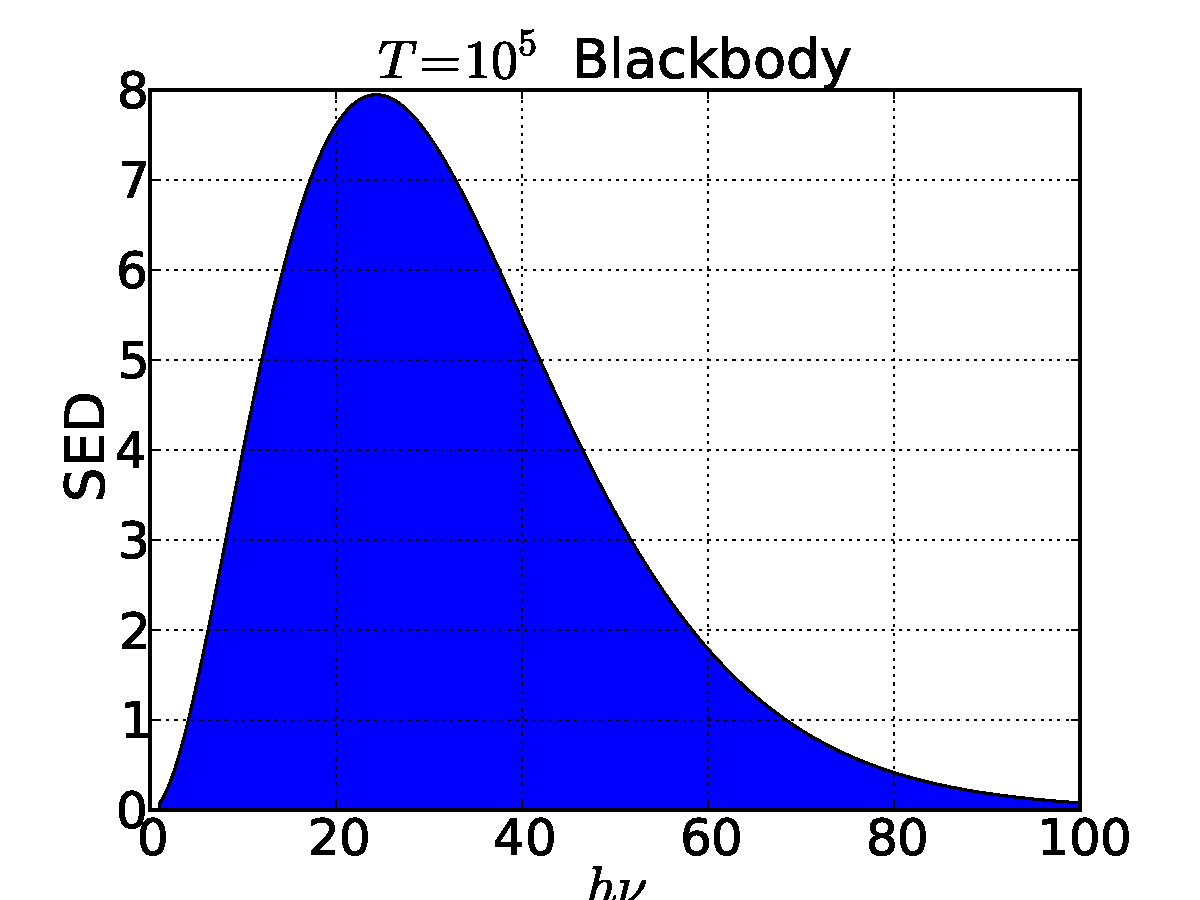
\includegraphics[scale=0.3, trim=1.0cm 0.5cm 1.25cm 0.5cm]{blackbody.pdf}
      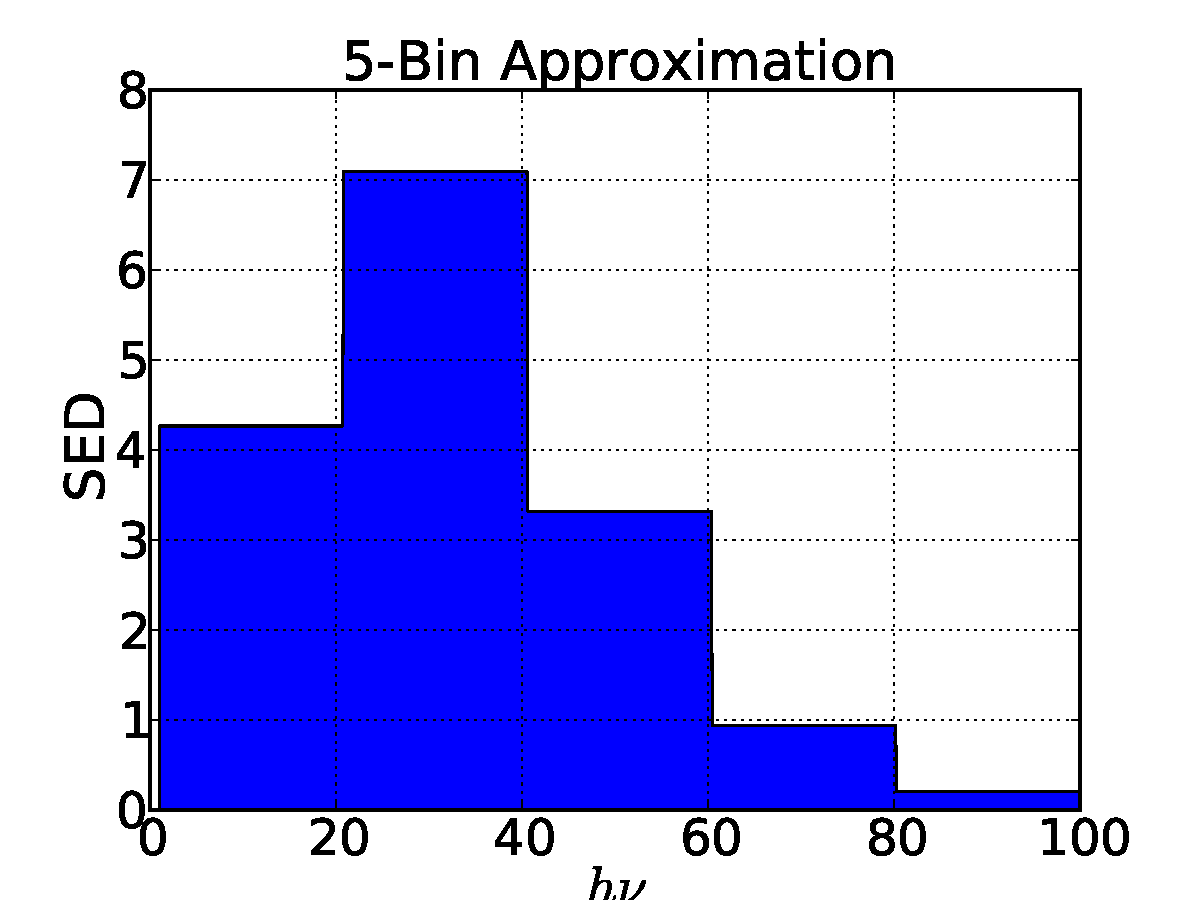
\includegraphics[scale=0.3, trim=1.0cm 0.5cm 1.25cm 0.5cm]{blackbody-5bin.pdf}
      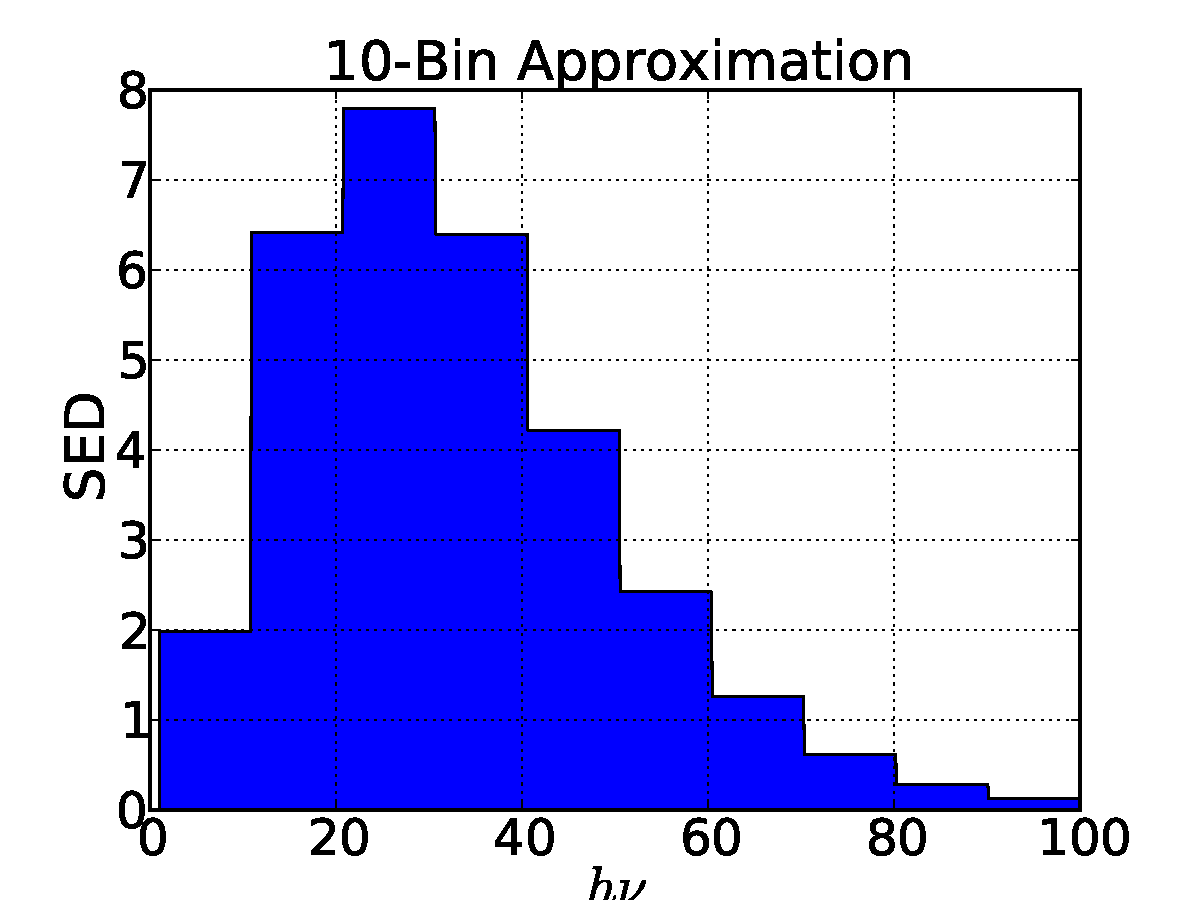
\includegraphics[scale=0.3, trim=1.0cm 0.5cm 1.25cm 0.5cm]{blackbody-10bin.pdf}
      \hfill}
    \caption{Comparison between true $T=10^5$ blackbody radiation
      spectral energy distribution and its contiguous 5 and 10 group
      counterparts.}  
    \label{fig:binned_blackbody}
  \end{figure}

\item[(iv)] This piecewise constant approximation of the underlying
  frequency dependence of $\Enu$ is only first-order accurate as a
  function of the bin width.

\item[(v)] Under this discretization, we also allow for gaps in the
  radiation spectrum (i.e. non-contiguous frequency bands).  For
  example, if one wanted a crude approximation to separately
  transporting both UV and X-ray radiation, a two-bin approach with
  $g_1 = [13.6,100)$ and $g_2 = [500,10000)$ could be used.

\item[(vi)] To ensure photon conservation, these bins must be filled
  with the total amount of $\Enu$ within each bin, {\em not} the
  value at the central frequency, i.e.
  \[
     E_{\omega}(t,\rvec) = \int_{\nu_{\omega,L}}^{\nu_{\omega,R}}
     \Enu(t,\rvec,\nu)\,\mathrm d\nu, \quad \omega=1,\ldots,N_f.
  \]
  This applies to both initial conditions, and (more importantly) to
  the emissivity values that source each radiation group.

\end{itemize}
With this approximation in place, we may consider the implications on
solving the radiation energy density equation
\eqref{eq:mgfld_simplified2}.  Due to the piecewise constant
radiation approximation, we simplify the equation
\eqref{eq:mgfld_simplified2} by integrating over each frequency
group.  As a result, instead of solving a single frequency-dependent equation
\eqref{eq:mgfld_simplified2}, we now have separate equations for each
radiation group. We investigate each term separately,
\begin{align}
 \label{eq:multigroup_timederivative}
   \partial_{t} \Enu &\;\rightarrow\;
   \int_{\nu_{\omega,L}}^{\nu_{\omega,R}} \partial_{t} \Enu\,\mathrm d\nu
   =
   \int_{\nu_{\omega,L}}^{\nu_{\omega,R}} \partial_{t} E_{\omega}\,\mathrm d\nu
   =
   \partial_{t} E_{\omega}, \\
 \label{eq:multigroup_diffusion}
   \nabla\cdot(D_{\nu}\,\nabla\Enu) &\;\rightarrow\;
   \int_{\nu_{\omega,L}}^{\nu_{\omega,R}} \nabla\cdot(D_{\nu}\,\nabla\Enu)\,\mathrm d\nu
   =
   \nabla\cdot(D_{\omega}\,\nabla E_{\omega}), \\
 \label{eq:multigroup_depletion}
   \frac{3 \adot}{a} \Enu &\;\rightarrow\;
   \int_{\nu_{\omega,L}}^{\nu_{\omega,R}} \frac{3 \adot}{a} \Enu\,\mathrm d\nu
   =
   \frac{3 \adot}{a} E_{\omega}, \\
 \label{eq:multigroup_emissivity}
   \eta_{\nu} &\;\rightarrow\;
   \int_{\nu_{\omega,L}}^{\nu_{\omega,R}} \eta_{\nu}\,\mathrm d\nu
   \equiv
   \eta_{\omega}, \\
 \label{eq:multigroup_opacity}
   c \kappa_{\nu} \Enu &\;\rightarrow\;
   \int_{\nu_{\omega,L}}^{\nu_{\omega,R}} c \kappa_{\nu} \Enu\,\mathrm d\nu
   =
   c E_{\omega}\left(\frac{1}{|g_{\omega}|} \int_{\nu_{\omega,L}}^{\nu_{\omega,R}} \kappa_{\nu}\,\mathrm d\nu\right)
   \equiv
   c E_{\omega} \kappa_{\omega},
\end{align}
where the equations \eqref{eq:multigroup_emissivity} and
\eqref{eq:multigroup_opacity} above define the multi-group emissivities
and opacities, $\eta_{\omega}$ and $\kappa_{\omega}$,
$\omega=1,\ldots,N_f$, respectively.

The remaining frequency coupling term is less trivial,
\begin{align}
\notag
   \frac{\nu \adot}{a}\partial_{\nu}\Enu \;\rightarrow\;
   \int_{\nu_{\omega,L}}^{\nu_{\omega,R}} \frac{\nu \adot}{a}\partial_{\nu}\Enu\,\mathrm d\nu
   &=
   \frac{\adot}{a} \int_{\nu_{\omega,L}}^{\nu_{\omega,R}} \nu\,\partial_{\nu}\Enu\,\mathrm d\nu \\
\label{eq:multigroup_redshifting}
   &=
   \frac{\adot}{a}
   \left[(\nu\,\Enu)\bigg\vert_{\nu_{\omega,L}}^{\nu_{\omega,R}} - \int_{\nu_{\omega,L}}^{\nu_{\omega,R}} \Enu\,\mathrm d\nu\right]\\
\notag
   &\approx
   \frac{\adot\, \nu_{\omega,R}}{2a}\left(\frac{E_{\omega}}{|g_{\omega}|} + \frac{E_{\omega+1}}{|g_{\omega+1}|}\right) -
   \frac{\adot\, \nu_{\omega,L}}{2a}\left(\frac{E_{\omega-1}}{|g_{\omega-1}|}+\frac{E_{\omega}}{|g_{\omega}|}\right) - 
   \frac{\adot}{a}E_{\omega}.
\end{align}
We note that derivation of the above term required integration by
parts, as well as approximation of the radiation energy density at the
bin frequency boundaries, 
\[
   \Enu(\nu_{\omega}) \approx \frac12\left(\frac{E_{\omega-1}}{|g_{\omega-1}|}+\frac{E_{\omega}}{|g_{\omega}|}\right), \qquad
   \Enu(\nu_{\omega+1}) \approx \frac12\left(\frac{E_{\omega}}{|g_{\omega}|} + \frac{E_{\omega+1}}{|g_{\omega+1}|}\right),
\]
which is only valid if the radiation groups $E_{\omega-1}$,
$E_{\omega}$ and $E_{\omega+1}$ are defined over contiguous bands,
i.e. if
\begin{equation}
\label{eq:contiguous_bands}
   \nu_{\omega-1,R} = \nu_{\omega,L} \quad\text{and}\quad
   \nu_{\omega,R} = \nu_{\omega+1,L}.
\end{equation}
Furthermore, this term accounts for redshifting effects due to
cosmological expansion, that pull radiation from higher frequencies
downward.  Although our multi-group radiation approximation is no
longer continuous as a function of frequency, rendering the partial
derivative $\partial_\nu\Enu$ undefined, we have used integration by
parts to instead consider this term as a radiation flux from
higher-frequency groups downward.  Furthermore, the first and last
radiation groups deserve special attention since they cannot have
left and right neighbors, respectively (as well as any other groups
that have a non-contiguous frequency band with a lower/higher group).
For these two groups, we instead approximate 
\begin{align}
 \label{eq:multigroup_redshifting_left}
   \int_{\nu_{1,L}}^{\nu_{1,R}} \frac{\nu \adot}{a}\partial_{\nu}\Enu\,\mathrm d\nu
   &\approx
   \frac{\adot\, \nu_{1,R}}{2a}\left(\frac{E_1}{|g_1|} + \frac{E_2}{|g_2|}\right) -
   \frac{\adot\, \nu_{1,L} E_1}{a|g_1|} - \frac{\adot}{a}E_1,
\\
 \label{eq:multigroup_redshifting_right}
   \int_{\nu_{N_f,L}}^{\nu_{N_f,R}} \frac{\nu \adot}{a}\partial_{\nu}\Enu\,\mathrm d\nu
   &\approx
   \frac{\adot\, \nu_{N_f,R} E_{N_f}}{a|g_{N_f}|} -
   \frac{\adot\, \nu_{N_f,L}}{2a}\left(\frac{E_{N_f-1}}{|g_{N_f-1}|}+\frac{E_{N_f}}{|g_{N_f}|}\right) - 
   \frac{\adot}{a}E_{N_f}.
\end{align}
We note that for intermediate radiation groups whose frequency bands
do not touch their ``neighbor'', we use similar formulas.  Similarly,
for isolated radiation groups that have no ``neighbors'', we instead
approximate this term as 
\begin{align}
 \label{eq:multigroup_redshifting_alone}
   \int_{\nu_{\omega,L}}^{\nu_{\omega,R}}
   \frac{\nu \adot}{a}\partial_{\nu}\Enu\,\mathrm d\nu 
   &\approx
   \frac{\adot\, \nu_{\omega,R}\, E_{\omega}}{a|g_{\omega}|} -
   \frac{\adot\, \nu_{\omega,L}\, E_{\omega}}{a|g_{\omega}|} - 
   \frac{\adot}{a}E_{\omega}.
\end{align}
Combining all of the above terms,
\eqref{eq:multigroup_timederivative}-\eqref{eq:multigroup_redshifting_alone},
our multi-group radiation energy density equations may be written as
\begin{align}
  \label{eq:mgfld_multigroup}
  \partial_{t} E_{\omega} - \nabla\cdot(D_{\omega}\,\nabla E_{\omega}) 
      + \frac{3 \adot}{a} E_{\omega} - (\Diamond)
    = \eta_{\omega} - c \kappa_{\omega} E_{\omega},\quad \omega=0,\ldots,N_f-1,
\end{align}
where $(\Diamond)$ corresponds to one of
\eqref{eq:multigroup_redshifting},
\eqref{eq:multigroup_redshifting_left},
\eqref{eq:multigroup_redshifting_right} or
\eqref{eq:multigroup_redshifting_alone}, depending on the contiguity
of the frequency bands surround $g_\omega$. 

To complete the model, we must determine the photo-heating and
photo-ionization terms that couple the radiation to the matter.  As
before, we utilize the integral form of their definitions, along with
the piecewise-constant definition of our radiation energy density
\eqref{eq:multigroup_radiation}.  

First, we compute the integrated photoionization rate $\Gamma_i^{ph}$
for each species $\mn_i$ as 
\begin{align}
\label{eq:multigroup_photoionization}
   \Gamma_i^{ph}(t,\rvec)  &= 
   c \int_{\bar{\nu}_i}^{\infty} \frac{\sigma_{\mn_i}(\nu)\Enu(t,\rvec,\nu)}{h\nu}\,\mathrm d\nu =  
   c \sum_{\omega=1}^{N_f} \int_{\nu_{\omega,L}}^{\nu_{\omega,R}} \frac{\sigma_{\mn_i}(\nu) E_{\omega}(t,\rvec)}{h\nu|g_{\omega}|}\,\mathrm d\nu \\
\notag
   &= \sum_{\omega=1}^{N_f} \frac{c E_{\omega}(t,\rvec)}{h}\,
   \left(\frac{1}{|g_{\omega}|} 
     \int_{\nu_{\omega,L}}^{\nu_{\omega,R}} \frac{\sigma_{\mn_i}(\nu)}{\nu}\,\mathrm d\nu\right), 
   \qquad i=1,\ldots,N_\text{chem},
\end{align}
where as with the multi-frequency model, we assume that the species
cross sections satisfy $\sigma_{\mn_i}(\nu) = 0$ for all $\nu <
\bar{\nu}_i$.

Similarly, we compute the specific photoheating rate as 
\begin{align}
\notag
   G(t,\rvec) &= 
   \frac{c}{\rhob} \sum_{i=1}^{N_\text{chem}} \mn_i
     \int_{\bar{\nu}_i}^{\infty} \sigma_{\mn_i}(\nu) \Enu(t,\rvec,\nu)
     \left(\frac{h\nu - h\bar{\nu}_i}{h\nu}\right)\,\mathrm d\nu \\
\label{eq:multigroup_photoheating}
     &= 
   \sum_{i=1}^{N_\text{chem}} \sum_{\omega=1}^{N_f} \frac{c\,\mn_i\, E_{\omega}(t,\rvec)}{\rhob} 
     \left(\frac{1}{|g_{\omega}|}\int_{\nu_{\omega,L}}^{\nu_{\omega,R}} \sigma_{\mn_i}(\nu) 
     \left(1 - \frac{\bar{\nu}_i}{\nu}\right)\,\mathrm d\nu\right).
\end{align}

We note that in both \eqref{eq:multigroup_photoionization} and
\eqref{eq:multigroup_photoheating}, we have the integrals 
\begin{align}
  \label{eq:integrals} 
    \frac{1}{|g_{\omega}|}\int_{\nu_{\omega,L}}^{\nu_{\omega,R}} \frac{\sigma_{\mn_i}(\nu)}{\nu}\,\mathrm d\nu
    \qquad\text{and}\qquad
    \frac{1}{|g_{\omega}|}\int_{\nu_{\omega,L}}^{\nu_{\omega,R}} \sigma_{\mn_i} \left(1 - \frac{\bar{\nu}_i}{\nu}\right)\,\mathrm d\nu.
\end{align}
Since these integrals depend only on the {\em a-priori} defined
radiation groups $g_{\omega}=[\nu_{\omega,L},\nu_{\omega,R})$ and species cross-sections
$\sigma_{\mn_i}$, we may compute these once at problem initialization
and reuse them throughout the simulation.  For each of these
integrals, we use an adaptive, high-order Gaussian quadrature
method for numerically approximating each integral, manually adjusting
any interval bounds to account for regions where $\sigma_i(\nu)=0$.




\section{Units in Enzo cosmology}
\label{sec:units}

When run with cosmological expansion enabled, Enzo modifies the
units of each internal field throughout the simulation to account for
cosmological expansion.  We define the comoving position $\xvec$
through the relationship $\rvec = \Lunit\xvec \propto a \xvec$
(specific details are below in equation \eqref{eq:Lunit}), where $a$
is the cosmological expansion factor.  This is a time-dependent
(equivalently, redshift-dependent) factor, satisfying the relationship
\begin{align}
  \label{eq:CurrentRedshift}
  z &= \frac{1}{a} - 1,
\end{align}
where $z$ is the current (time-dependent) redshift.  We note that
since $z$ decreases as time proceeds, $a$ increases as a function of
time, since 
\begin{align}
  \label{eq:expansion_factor}
  a = \frac{1}{1+z}.
\end{align}

Enzo then defines the unit non-dimensionalization factors:
\begin{align}
  \label{eq:Dunit}
  \Dunit &= (1.88\times10^{-29}) \Omega_{mn} H_{cn}^2 (1 + z)^3, \\
  \label{eq:Lunit}
  \Lunit &= \frac{(3.086\times10^{24}) L_c}{H_{cn} (1 + z)}
          \qquad \left(\text{i.e.}\quad \Lunit = \frac{(3.086\times10^{24}) L_c}{H_{cn}}a\right), \\
  \label{eq:Tunit}
  \Tunit &= \frac{2.52\times10^{17}}{\Omega_{mn}^{1/2} H_{cn} (1 + z_I)^{3/2}}, \\
  \label{eq:Vunit}
  \Vunit &= (1.225\times10^{7}) L_c \sqrt{\Omega_{mn}(1 + z_I)}, \\
  \label{eq:Aunit}
  \Aunit &= (1+z_I)^{-1}.
\end{align}
Here $a = \Aunit \tA$, where $\tA$ is Enzo's normalized value,  
$\Omega_{mn}$ is Enzo's {\tt OmegaMatterNow} parameter, 
$H_{cn}$ is Enzo's {\tt HubbleConstantNow} parameter, 
$z_I$ is Enzo's {\tt InitialRedshift} parameter, and
$L_c$ is Enzo's {\tt ComovingBoxSize} parameter.
As a result, Enzo actually computes the current redshift via the
formula 
\begin{align}
  \label{eq:CurrentRedshiftFormula}
  z &= \frac{1 + z_I}{\tA} - 1.
\end{align}
We note that under these definitions, $\Vunit \ne \Lunit / \Tunit$, since
\begin{align*}
   \frac{\Lunit}{\Tunit} &= 
   \frac{(3.086\times10^{24}) L_c \left(\Omega_{mn}^{1/2} H_{cn} (1 + z_I)^{3/2}\right)}
         {H_{cn} (1 + z)\left(2.52\times10^{17}\right)} \\
   &= 
   (1.2246\times10^{7}) L_c \sqrt{\Omega_{mn}(1 + z_I)} \frac{(1 + z_I)}{(1 + z)},
\end{align*}
which differs from $\Vunit$ both in the precision of the leading
constant (minor difference) and also by a factor of $(1+z_I)/(1+z)$, that grows
in magnitude as time proceeds, especially for simulations having large
initial redshift (major difference).

With these unit normalization factors defined, we may also consider a
unit normalization factor for radiation energy density, that can be
defined as either 
\[
  \Dunit \Vunit^2, \quad\text{or}\quad 
  \Dunit \frac{\Lunit^2}{\Tunit^2},
\]
since both constitute the correct CGS units.  However, since in
cosmological simulations $\Vunit \ne \Lunit / \Tunit$, these two
definitions are not the same.  We choose the first of these,
\begin{equation}
  \label{eq:Eunit}
  \Eunit = \Dunit \Vunit^2.
\end{equation}

We note that even when run without cosmology, unit scaling factors may
be defined within Enzo for running a simulation.  In this case, we
similarly use Enzo's internal unit scaling factors to define the
radiation unit scaling factor, $\Eunit$. 





\section{Recasting to comoving, normalized form}
\label{sec:comoving_eqn}

Our equations \eqref{eq:mgfld_multifrequency},
\eqref{eq:mgfld_multigroup} and
\eqref{eq:Morel_limiterD}-\eqref{eq:Morel_limiterR} are valid in
proper CGS units, whereas Enzo's fields are stored in comoving,
normalized form.  Specifically, the terms in our equations relate to
Enzo's comoving, normalized terms in the following manner: 
\begin{itemize}
\item $\rhob = \Dunit \tRho$, where $\rhob$ is the proper, CGS
  density, and $\tRho$ is Enzo's comoving, normalized
  density value,
\item $\vb = \Vunit \tilde{\vb}$, where $\vb$ is the proper peculiar
  baryonic CGS velocity, and $\tilde{\vb}$ is Enzo's comoving,
  normalized velocity value,
\item $e = \Vunit^2 \tilde{e}$, where $e$ is the proper
  baryonic energy per unit mass, and $\tilde{e}$ is Enzo's comoving,
  normalized energy value,
\item $E_{\omega} = \Eunit \tE$, where $E_{\omega}$ is the proper, CGS radiation
  energy (monochromatic or group), and $\tE_{\omega}$ is Enzo's comoving,
  normalized radiation energy value for the specified frequency or
  group,
\item $a = \Aunit \tA$, as described above in equation
  \eqref{eq:Aunit},
\item $\adot = \left(\Aunit/\Tunit\right) \dot{\tA}$, where $\adot$ is
  the true cosmological expansion rate, and $\dot{\tA}$ is Enzo's
  normalized value,
\item $\rvec = \Lunit \xvec$, where $\rvec$ is the
  proper, CGS position, and $\xvec$ is Enzo's comoving normalized position,
\item $t = \Tunit \tT$, where $t$ is the CGS time, and $\tT$ is Enzo's
  normalized time,
\item $\kappa_{\omega} = \tK_{\omega} \Kunit$, where $\kappa_{\omega}$ is the proper, CGS
  opacity for the $\omega$-th frequency or group, $\tK_{\omega}$ is Enzo's
  normalized value, and $\Kunit \propto \Lunit^{-1}$.
\end{itemize}

We also note that in order for us to convert our equations
for the proper CGS radiation energy ($E_{\omega}$) to the normalized,
comoving radiation energy density ($\tE_{\omega}$) we must consider how our
time derivative must be modified.  Specifically, since $E_{\omega} = \Eunit
\tE_{\omega}$, then by the product rule,
\[
   \partial_t E_{\omega} = \partial_t \left(\Eunit \tE_{\omega}\right) = 
   \Eunit\, \partial_t \tE_{\omega} + \tE_{\omega}\, \partial_t \Eunit.
\]
Due to our choice of $\Eunit = \Dunit \Vunit^2 \propto (1+z)^3$, we then have 
\[
   \partial_t \Eunit = \frac{3\, \Eunit\, \partial_t z}{1+z}.
\]
Moreover, because $z = \frac{1}{a}-1$ we have $\partial_t z =
-\frac{\adot}{a^2}$, and since $a = \frac{1}{1+z}$, this becomes 
\[
   \partial_t \Eunit = -3\Eunit\frac{\adot}{a}.
\]
As a result, we have 
\begin{align*}
   \partial_t E_{\omega} &= \Eunit\, \partial_t \tE_{\omega} - 3\Eunit \frac{\adot}{a} \tE_{\omega} \\
   &= \Eunit\, \partial_t \tE_{\omega} - 3\frac{\adot}{a} E_{\omega},
\end{align*}
which will cancel the term $3 \frac{\adot}{a} E_{\omega}$ in either of the
equations \eqref{eq:mgfld_multifrequency} or
\eqref{eq:mgfld_multigroup}.  Specifically, after dividing through by 
$\Eunit$ and canceling like terms, the multi-frequency equation
\eqref{eq:mgfld_multifrequency} may instead be written in terms of the
comoving, normalized radiation energy density: 
\begin{align}
  \label{eq:mgfld_multifrequency_Ecomoving}
  \partial_{t} \tE_{\omega} - \nabla\cdot(D_{\omega}\,\nabla \tE_{\omega}) 
    = \frac{\eta_{\omega}}{\Eunit} - c \kappa_{\omega} \tE_{\omega}, \qquad \omega=0,\ldots,N_f.
\end{align}
Similarly, the multi-group equation \eqref{eq:mgfld_multigroup} can be
written in comoving, normalized for as:
\begin{align}
  \label{eq:mgfld_multigroup_Ecomoving}
  \partial_{t} \tE_{\omega} - \nabla\cdot(D_{\omega}\,\nabla \tE_{\omega}) +
    \frac{\adot}{a}\tE_{\omega} - (\square)_{\omega} = \frac{\eta_{\omega}}{\Eunit} - c
    \kappa_{\omega} \tE_{\omega}, \quad \omega=0,\ldots,N_f-1,
\end{align}
where we now define $(\square)_{\omega}$ as 
\begin{equation}
\label{eq:square_omega}
  (\square)_{\omega} = \begin{cases}
    \frac{\adot}{2a|g_{\omega}|}\left(
      \nu_{\omega+1} (\tE_{\omega}+\tE_{\omega+1}) - 2\nu_{\omega} \tE_{\omega}\right),&
      \text{if}\quad \omega=0,\\
    \frac{\adot}{2a|g_{\omega}|}\left(
      2\nu_{\omega+1} \tE_{\omega} - \nu_{\omega} (\tE_{\omega-1}+\tE_{\omega})\right),&
      \text{if}\quad \omega=N_f-1,\\
    \frac{\adot}{2a|g_{\omega}|}\left(
      \nu_{\omega+1} (\tE_{\omega}+\tE_{\omega+1}) - \nu_{\omega}(\tE_{\omega-1}+\tE_{\omega})\right),& 
      \text{otherwise}.
  \end{cases}
\end{equation}


Similarly, since the proper position changes as a function of time,
then we may consider spatial differentiation with respect to the
normalized comoving position $\xvec$.  Since 
\[
   \rvec = \Lunit \xvec \quad\Longleftrightarrow\quad
   \xvec = \frac{\rvec}{\Lunit},
\]
then the chain rule dictates that
\[
   \frac{\partial}{\partial \rvec} \ = \
   \frac{\partial \xvec}{\partial \rvec}
   \frac{\partial}{\partial \xvec} \ = \
   \frac{1}{\Lunit}\frac{\partial}{\partial \xvec}.
\]
We therefore denote the comoving, normalized differentiation operator
as $\tnabla$, such that 
\[
   \nabla = \frac{1}{\Lunit}\tnabla.
\]
Resultingly, upon converting \eqref{eq:mgfld_multifrequency_Ecomoving}
to comoving, normalized units, we have the multi-frequency equation
\begin{align}
  \label{eq:mgfld_multifrequency_comoving}
  \partial_{t} \tE_{\omega} - \frac{1}{\Lunit^2}\tnabla\cdot\(D_{\omega}\,\tnabla \tE_{\omega}\)
    = \frac{\eta_{\omega}}{\Eunit} - c\kappa_{\omega} \tE_{\omega}, \quad \omega=0,\ldots,N_f,
\end{align}
and converting \eqref{eq:mgfld_multigroup_Ecomoving} we obtain the
multi-group equation 
\begin{align}
  \label{eq:mgfld_multigroup_comoving}
  \partial_{t} \tE_{\omega} - \frac{1}{\Lunit^2}\tnabla\cdot(D_{\omega}\,\tnabla \tE_{\omega}) +
    \frac{\adot}{a}\tE_{\omega} - (\square)_{\omega} = \frac{\eta_{\omega}}{\Eunit} - c
    \kappa_{\omega} \tE_{\omega}, \quad \omega=0,\ldots,N_f-1.
\end{align}

Similarly, we may consider time differentiation with respect to the
normalized time value, $\tT$:
\[
   \frac{\partial}{\partial t} \ = \
   \frac{\partial \tT}{\partial t} \frac{\partial}{\partial \tT} \ = \
   \frac{1}{\Tunit}\frac{\partial}{\partial \tT}.
\]
Inserting this into \eqref{eq:mgfld_multifrequency_comoving} we have
the multi-frequency equations
\begin{align}
  \label{eq:mgfld_multifrequency_tnormalized}
  \partial_{\tT} \tE_{\omega} - \frac{\Tunit}{\Lunit^2}\tnabla\cdot\(D_{\omega}\,\tnabla \tE_{\omega}\)
    = \frac{\Tunit\eta_{\omega}}{\Eunit} - \Tunit c\kappa_{\omega} \tE_{\omega}, \quad \omega=0,\ldots,N_f,
\end{align}
and inserting into \eqref{eq:mgfld_multigroup_comoving} we have the
corresponding multi-group version,
\begin{align}
  \label{eq:mgfld_multigroup_tnormalized}
  \partial_{\tT} \tE_{\omega} - \frac{\Tunit}{\Lunit^2}\tnabla\cdot(D_{\omega}\,\tnabla \tE_{\omega}) +
    \frac{\Tunit\adot}{a}\tE_{\omega} - \Tunit(\square)_{\omega} = \frac{\Tunit\eta_{\omega}}{\Eunit} - 
    \Tunit c \kappa_{\omega} \tE_{\omega}, \quad \omega=0,\ldots,N_f-1.
\end{align}


Lastly, we will convert these equations so that they depend only on
Enzo's normalized variables, $\tT$, $\tE_{\omega}$, $\tA$, $\dot{\tA}$ and
$\tK_{\omega}$.  To this end, we expand each variable in terms of its
normalized value and unit factor.  We begin with the multi-frequency
equations: 
\begin{align}
  \label{eq:mgfld_multifrequency_comoving_normalized}
  &\partial_{\tT} \tE_{\omega} - \frac{\Tunit}{\Lunit^2}\tnabla\cdot\(D_{\omega}\,\tnabla \tE_{\omega}\)
    = \frac{\Tunit\,\eta_{\omega}}{\Eunit} - \Tunit\, \Kunit\, c\, \tK_{\omega}\, \tE_{\omega}, \quad
    \omega=0,\ldots,N_f,
\end{align}
where we compute the limiter as
\begin{align}
  \label{eq:Morel_limiterD_normalized}
  D_{\omega,i} &= c \left(9\tK_{\omega}^2\Kunit^2 +
  R_{\omega,i}^2\right)^{-1/2}, \quad i=1,2,3,\quad \omega=0,\ldots,N_f\\
  \label{eq:Morel_limiterR_normalized}
  R_{\omega,i} &= \frac{|\partial_{\xvec_i}\tE_{\omega}|}{\Lunit \tE_{\omega}}, \quad i=1,2,3,\quad \omega=0,\ldots,N_f.
\end{align}


Similarly, for the multi-group equations, we have for each $\omega=0,\ldots,N_f-1$,
\begin{align}
  \notag
  &\partial_{\tT} \tE_{\omega} - \frac{\Tunit}{\Lunit^2}\tnabla\cdot\(D_{\omega}\,\tnabla \tE_{\omega}\)
    + \frac{\Tunit \Aunit\tAdot}{\Tunit \Aunit\tA} \tE_{\omega} - \Tunit(\square)_{\omega} = 
    \frac{\Tunit\eta_{\omega}}{\Eunit} - \Tunit\, \Kunit\, c\, \tK_{\omega}\, \tE_{\omega},\\
  \Leftrightarrow \quad & \\
  \label{eq:mgfld_multigroup_comoving_normalized}
  &\partial_{\tT} \tE_{\omega} - \frac{\Tunit}{\Lunit^2}\tnabla\cdot\(D_{\omega}\,\tnabla \tE_{\omega}\)
    + \frac{\tAdot}{\tA} \tE_{\omega} - (\tilde{\square})_{\omega} = 
    \frac{\Tunit\eta_{\omega}}{\Eunit} - \Tunit\, \Kunit c\, \tK_{\omega}\, \tE_{\omega},
\end{align}
with the limiter the same as in
\eqref{eq:Morel_limiterD_normalized}-\eqref{eq:Morel_limiterR_normalized},
and where we compute $(\tilde{\square})_{\omega}$ as
\begin{equation}
\label{eq:square_omega_normalized}
  (\tilde{\square})_{\omega} = \begin{cases}
    \frac{\tAdot}{2\tA|g_{\omega}|}\left(
      \nu_{\omega+1} (\tE_{\omega}+\tE_{\omega+1}) - 2\nu_{\omega} \tE_{\omega}\right),&
      \text{if}\quad \omega=0,\\
    \frac{\tAdot}{2\tA|g_{\omega}|}\left(
      2\nu_{\omega+1} \tE_{\omega} - \nu_{\omega} (\tE_{\omega-1}+\tE_{\omega})\right),&
      \text{if}\quad \omega=N_f-1,\\
    \frac{\tAdot}{2\tA|g_{\omega}|}\left(
      \nu_{\omega+1} (\tE_{\omega}+\tE_{\omega+1}) - \nu_{\omega}(\tE_{\omega-1}+\tE_{\omega})\right),& 
      \text{otherwise}.
  \end{cases}
\end{equation}





\section{Finite volume PDE approximation}
\label{sec:fv_approximation}

We define the spatially-discretized version of our equations in the
context of a uniform (i.e.~non-AMR) mesh with comoving grid spacings $\Delta x$,
$\Delta y$ and $\Delta z$; as the AMR extensions of this involve a
standard extension of the same equation over patches with smaller mesh
size, the uniform grid assumption will prove sufficient for this
derivation.  On this uniform grid, we define the finite volume cell
centers at the grid points in comoving, normalized units as: 
\begin{align*}
   \xvec_{i,j,k} &= \left[\,x_i,\,  y_j,\, z_k\,\right], \\
   x_i &= \left(i + \tfrac12\right) \Delta x, \\
   y_j &= \left(j + \tfrac12\right) \Delta y, \\
   z_k &= \left(k + \tfrac12\right) \Delta z.
\end{align*}
Enzo's data arrays contain the discrete values of each field over the
simulation volume at each of these grid points.  More specifically,
Enzo uses three-dimensional data arrays to store these discretized
solution values at specific points in time.  We denote $\tE^n_{\omega,i,j,k}$
as our approximation to the comoving and normalized solution at the
normalized time $\tT_{n}$ and at the comoving normalized spatial
location $\xvec_{i,j,k}$ (and do similarly for the other field data).
We must therefore consider how to discretize the space and time
derivatives of our equations
\eqref{eq:mgfld_multifrequency_comoving_normalized} and 
\eqref{eq:mgfld_multigroup_comoving_normalized}
so that they depend on only these discrete data values.

We first separate the space and time discretizations.  First, we
discretize in time using a one-step $\theta$-method.  Introducing the
notation 
\[
   \mD_{\omega}(\tE_{\omega},\tK_{\omega},\eta_{\omega},\tA,\tAdot) = 
   \frac{\Tunit}{\Lunit^2}\tnabla\cdot\(D_{\omega}\,\tnabla \tE_{\omega}\)
    + \frac{\Tunit\eta_{\omega}}{\Eunit} 
    - \Tunit \Kunit\, c\, \tK_{\omega}\, \tE_{\omega}
\]
for the multi-frequency equation
\eqref{eq:mgfld_multifrequency_comoving_normalized}, or 
\[
   \mD_{\omega}(\tE_{\omega},\tK_{\omega},\eta_{\omega},\tA,\tAdot) = 
   \frac{\Tunit}{\Lunit^2}\tnabla\cdot\(D_{\omega}\,\tnabla \tE_{\omega}\)
    - \frac{\tAdot}{\tA} \tE_{\omega} + (\tilde{\square})_{\omega}
    + \frac{\Tunit\eta_{\omega}}{\Eunit} 
    - \Tunit \Kunit\, c\, \tK_{\omega}\, \tE_{\omega}
\]
for the multi-group equation \eqref{eq:mgfld_multigroup_comoving_normalized},
and denoting $\tE_{\omega}^n$ as our approximation to the spatially continuous
solution at time $\tT_{n}$, the $\theta$-method for both equations
\eqref{eq:mgfld_multifrequency_comoving_normalized} and
\eqref{eq:mgfld_multigroup_comoving_normalized} may be written as
\begin{align}
  \label{eq:mgfld_theta}
  \tE_{\omega}^{n+1} - \tE_{\omega}^n &= 
    \theta\Delta \tT \mD(\tE_{\omega}^{n+1},\tK_{\omega}^{n+1},\eta_{\omega}^{n+1},\tA^{n+1},\tAdot^{n+1}) 
    + (1-\theta)\Delta \tT \mD(\tE_{\omega}^n,\tK_{\omega}^n,\eta_{\omega}^n,\tA^n,\tAdot^n),
\end{align}
where in the first $\mD$ term we lag the implicit dependence of the
solution on the flux limiter $D_{\omega}^{n+1}$ to the previous time, $D_{\omega}^n$ to
result in a linearly implicit system of equations.  

We must similarly apply our finite-volume spatial discretization of
the operator $\mD_{\omega}$.  For the discretized equation for
frequency/group $\omega$, centered at the comoving normalized spatial
position $\xvec_{i,j,k}$, we have  
\begin{align}
  \label{eq:mgfld_discrete}
  \tE_{\omega,i,j,k}^{n+1} - \tE_{\omega,i,j,k}^n &= \theta\Delta \tT \mD_{\omega,i,j,k}^{n+1} 
    + (1-\theta)\Delta \tT \mD_{\omega,i,j,k}^{n},
\end{align}
where for the multi-frequency equations
\begin{align}
  \label{eq:discrete_multifrequency_operator}
  \mD_{\omega,i,j,k} &= 
       \frac{\Tunit}{\Lunit^2 \Delta x^2}\(D_{\omega,i+1/2,j,k}\(\tE_{\omega,i+1,j,k} - \tE_{\omega,i,j,k}\) - D_{\omega,i-1/2,j,k}\(\tE_{\omega,i,j,k} - \tE_{\omega,i-1,j,k}\)\) \\
 \notag
    &+ \frac{\Tunit}{\Lunit^2 \Delta y^2}\(D_{\omega,i,j+1/2,k}\(\tE_{\omega,i,j+1,k} - \tE_{\omega,i,j,k}\) - D_{\omega,i,j-1/2,k}\(\tE_{\omega,i,j,k} - \tE_{\omega,i,j-1,k}\)\) \\
  \notag
    &+ \frac{\Tunit}{\Lunit^2 \Delta z^2}\(D_{\omega,i,j,k+1/2}\(\tE_{\omega,i,j,k+1} - \tE_{\omega,i,j,k}\) - D_{\omega,i,j,k-1/2}\(\tE_{\omega,i,j,k} - \tE_{\omega,i,j,k-1}\)\) \\
  \notag
    &+ \frac{\Tunit \eta_{\omega,i,j,k}}{\Eunit} 
     - \Tunit \Kunit\, c\, \tK_{\omega,i,j,k} \tE_{\omega,i,j,k},
\end{align}
and for the multi-group equations
\begin{align}
  \label{eq:discrete_multigroup_operator}
  \mD_{\omega,i,j,k} &= 
       \frac{\Tunit}{\Lunit^2 \Delta x^2}\(D_{\omega,i+1/2,j,k}\(\tE_{\omega,i+1,j,k} - \tE_{\omega,i,j,k}\) - D_{\omega,i-1/2,j,k}\(\tE_{\omega,i,j,k} - \tE_{\omega,i-1,j,k}\)\) \\
 \notag
    &+ \frac{\Tunit}{\Lunit^2 \Delta y^2}\(D_{\omega,i,j+1/2,k}\(\tE_{\omega,i,j+1,k} - \tE_{\omega,i,j,k}\) - D_{\omega,i,j-1/2,k}\(\tE_{\omega,i,j,k} - \tE_{\omega,i,j-1,k}\)\) \\
  \notag
    &+ \frac{\Tunit}{\Lunit^2 \Delta z^2}\(D_{\omega,i,j,k+1/2}\(\tE_{\omega,i,j,k+1} - \tE_{\omega,i,j,k}\) - D_{\omega,i,j,k-1/2}\(\tE_{\omega,i,j,k} - \tE_{\omega,i,j,k-1}\)\) \\
  \notag
    &- \frac{\tAdot}{\tA} \tE_{\omega,i,j,k} + (\tilde{\square})_{\omega,i,j,k} 
     + \frac{\Tunit \eta_{\omega,i,j,k}}{\Eunit} 
     - \Tunit \Kunit\, c\, \tK_{\omega,i,j,k} \tE_{\omega,i,j,k},
\end{align}
with
\begin{equation}
\label{eq:square_omega_normalized_discretized}
  (\tilde{\square})_{\omega,i,j,k} = \begin{cases}
    \frac{\tAdot}{2\tA|g_{\omega}|}\left(
      \nu_{\omega+1} (\tE_{\omega,i,j,k}+\tE_{\omega+1,i,j,k}) - 2\nu_{\omega} \tE_{\omega,i,j,k}\right),&
      \text{if}\quad \omega=0,\\
    \frac{\tAdot}{2\tA|g_{\omega}|}\left(
      2\nu_{\omega+1} \tE_{\omega,i,j,k} - \nu_{\omega} (\tE_{\omega-1,i,j,k}+\tE_{\omega,i,j,k})\right),&
      \text{if}\quad \omega=N_f-1,\\
    \frac{\tAdot}{2\tA|g_{\omega}|}\left(
      \nu_{\omega+1} (\tE_{\omega,i,j,k}+\tE_{\omega+1,i,j,k}) - \nu_{\omega}(\tE_{\omega-1,i,j,k}+\tE_{\omega,i,j,k})\right),& 
      \text{otherwise}.
  \end{cases}
\end{equation}
In the above, we must discretize the limiter at the faces
$\{(i\pm\frac12,j,k),(i,j\pm\frac12,k),(i,j,k\pm\frac12)\}$.
Furthermore, due to the limitations of floating-point arithmetic we
must enforce bounds on the calculations within the limiter to avoid
overflow errors.  With these constraints in mind, we discretize the
limiter as, e.g.
\begin{align}
  \label{eq:discrete_limiter}
  D_{\omega,i+1/2,j,k} &= \min\left\{ c \left(9\kappa_{\omega,i+1/2,j,k}^2 + R_{\omega,i+1/2,j,k}^2\right)^{-1/2},
    D_\text{max} \right\},\\
  \notag
  R_{\omega,i+1/2,j,k} &= \max\left\{\frac{2}{\Lunit \Delta x} \frac{|\tE_{\omega,i+1,j,k}-\tE_{\omega,i,j,k}|}{\tE_{\omega,i+1,j,k}+\tE_{\omega,i,j,k}}, R_\text{min} \right\}, \\
  \notag
  \kappa_{\omega,i+1/2,j,k} &= \frac{2 \tK_{\omega,i+1,j,k} \tK_{\omega,i,j,k}}{\tK_{\omega,i+1,j,k} + \tK_{\omega,i,j,k}}\Kunit.
\end{align}
While the limiter formulation shown here is somewhat standard in the
field, some of these specific implementation details have proven
difficult to master, which we will point out here.  First, through
significant trial and error, we have found that the limiter
bounds $R_\text{min}=10^{-20} \Lunit^{-1}$ and 
$D_\text{max}=10^{-2}\, c\, \Lunit$ provide the most robust results
in a wide range of simulations, including ``lab-frame''
radiation-hydrodynamics test problems, ``medium-scale'' astrophysical
simulations, and ``large-scale'' cosmological reionization
simulations.  The user may over-ride the constants $10^{-20}$ and
$10^{-2}$ in these definitions if desired, as described in Section
\ref{sec:user_interface}.  Second, we note that the face-centered
radiation field ($\tE_{\omega,i+1/2,j,k}$) and the face-centered
opacity ($\kappa_{\omega,i+1/2,j,k}$) are computed differently.  In
computing the face-centered radiation field (denominator of
$R_{\omega,i+1/2,j,k}$) we use the arithmetic mean of the neighboring 
cell-centered quantities, however in computing the face-centered
opacity we use the harmonic mean of the cell-centered quantities.
While theoretically both are equally valid, our experience has shown
that these approaches give the most robust results in cosmological
ionization simulations, wherein opacities may differ by orders of
magnitude in neighboring cells.

Finally, we note that in many of the above factors within equations
\eqref{eq:mgfld_discrete}-\eqref{eq:discrete_limiter} , the unit
values may change as a function of time due to cosmological expansion.
As a result, all quantities are converted using the unit evaluated at
the appropriate time step, $t_{n+1}$ or $t_n$.




\section{Enzo User Interface}
\label{sec:user_interface}

We anticipate to offer the following user interface for control over
the AMR-FLD solver for Enzo simulations.

Physics input parameters:
\begin{itemize}
\item {\em AMRFLDNumRadiationFields} -- integer denoting the number of
  radiation fields, $E_{\omega}$.  Default: 1
\item {\em AMRFLDFrequencyBand[:]}  -- pair of floating-point values
  denoting the frequency band for the specified radiation group.  If
  the upper limit is less than or equal to the lower limit, then the
  field is considered monochromatic at the lower bound frequency.  For
  example,
  \begin{verbatim}
     AMRFLDFrequencyBand[0] = 13.6 24.4
     AMRFLDFrequencyBand[1] = 54.4 54.4
     AMRFLDFrequencyBand[2] = 100.0 99.0
  \end{verbatim}
  specifies three frequency bands:
  \begin{itemize}
  \item[0] this radiation field spans the frequencies 13.6 to 24.4 eV,
  \item[1] this radiation field is monochromatic, at the frequency
    54.4 eV,
  \item[2] this radiation field is monochromatic, at the frequency
    100.0 eV.
  \end{itemize}
  A user must supply {\em AMRFLDNumRadiationFields} of these pairs,
  and they must be ordered by increasing frequencies (i.e we could
  not reorder the fields in the above example).  Additionally, the
  fields may not overlap (although neighboring non-monochromatic group
  bands may share a boundary).  For all fields that are adjacent, the
  redshifting terms present in equation
  \eqref{eq:square_omega_normalized_discretized} will be applied.
\item {\em AMRFLDNumSources} -- integer specifying the number of
  ionization sources to be specified in the input file (as opposed to
  on-the-fly by star-maker or other routines).
\item {\em AMRFLDSourceLocation[:]} -- set of three floating-point
  values specifying the location of each source (in normalized code
  units).
\item {\em AMRFLDSourceType[:]} -- integer flag denoting a pre-defined
  SED to use for all emissivity from a given source.
\item {\em AMRFLDSourceEnergy[:]} -- floating-point value specifying
  the total radiation emitted by a given source.  Must be used in
  combination with {\em AMRFLDSourceType[:]}.  At solver
  initialization, the SED will be numerically integrated over each
  radiation frequency band $[\nu_i, \nu_{i+1}]$ to determine each
  group's fraction of the {\em AMRFLDSourceEnergy[:]} for the source.
\item {\em AMRFLDSourceGroupEnergy[:][:]} -- may be used in lieu of the
  two previous parameters, {\em AMRFLDSourceType[:]} and {\em 
    AMRFLDSourceEnergy[:]}.  Specifies a floating-point value
  for the total energy of a specific source for a specific
  frequency/group (in physical units of ergs cm$^{-3}$ s$^{-1}$).  The
  first index is the source index, the second is the frequency/group
  index.
\item {\em AMRFLDLimiterRmin} -- floating point value specifying the
  dimensionless constant in the definition of $R_{\text{min}}$ in
  equation \eqref{eq:discrete_limiter}.  {\em Modify at your own
    risk.}  Default: $10^{-20}$.
\item {\em AMRFLDLimiterDmax} -- floating point value specifying the
  dimensionless constant in the definition of $D_{\text{max}}$ in
  equation \eqref{eq:discrete_limiter}.  {\em Modify at your own
    risk.}  Default: $10^{-2}$.
\end{itemize}


User requirements:
\begin{itemize}
\item Fields -- the problem initializer or provided restart file must
  allocate radiation and emissivity fields for each frequency or
  group.  These are expected to reside in the Enzo baryon fields 
  {\em RadiationFreq0} $\to$ {\em RadiationFreq9} and 
  {\em Emissivity0} $\to$ {\em Emissivity9}.  Of course, in actuality
  only {\em 2*AMRFLDNumRadiationFields} of these fields needs to be
  allocated, so simulations with fewer frequencies/groups can allocate
  only what they will need.

  In addition, the user must allocate the baryon fields {\em kphHI,
  kphHeI, kphHeII, PhotoGamma} and {\em kdissH2I} to enable communication 
  of photo-ionization and photo-heating rates from the AMR-FLD solver and 
  Enzo's chemistry and cooling routines.

\item Emissivities -- For problems in which the set of emission
  sources is unknown at run-time and cannot be specified in the input
  parameter file, the user is responsible for filling the emissivity
  fields {\em Emissivity0} $\to$ {\em Emissivity9}.  These should be
  filled in accordance with formulas
  \eqref{eq:multifrequency_emissivity} for multi-frequency
  simulations, or \eqref{eq:multigroup_emissivity} for multi-group
  simulations.  These fields should be filled using standard CGS units
  of ergs cm$^{-3}$ s$^{-1}$.

  We are considering the possibility of allowing a user-specified SED
  function, that at solver initialization will be numerically
  integrated over each radiation frequency band, with the resulting
  fractional areas of each band returned to the user.  This would
  allow for simplified on-the-fly decomposition of stellar energy into
  separate emissivities for each radiation group.
\end{itemize}


Solver input parameters:
\begin{itemize}
\item to be added
\end{itemize}



\bibliography{sources}
\bibliographystyle{siam}
\end{document}
